\documentclass{article}
\usepackage[final]{nips_2017}
\usepackage[utf8]{inputenc} % allow utf-8 input
\usepackage[T1]{fontenc}    % use 8-bit T1 fonts
\usepackage{hyperref}       % hyperlinks
\usepackage{url}            % simple URL typesetting
\usepackage{booktabs}       % professional-quality tables
\usepackage{amsfonts}       % blackboard math symbols
\usepackage{nicefrac}       % compact symbols for 1/2, etc.
\usepackage{microtype}      % microtypography
\usepackage{graphicx}
\title{Family kinship Recognition Using Deep Learning}

\author{
  Bruce Jianye Liu\\
  Department of Computer Science\\
  Stanford University\\
  \texttt{bruceliu@stanford.edu} \\
}

\begin{document}
% \nipsfinalcopy is no longer used

\begin{center}

\includegraphics[width=3cm, height=0.7cm]{CS230}
\end{center}

\maketitle

\section{Problem Description}
Half of genetic information is passed down from parents to children. Therefore
people biologically related share delicate similiarities. This declicacy could
be caught by human eyes, by looking at family photos. While computer vision
performance improving in the decade, it becomes impossible to use deep learning
model to capture the different. Kinship recognition could lead variety of
usefull applications in reality such as missing-children and parents matching,
family album organization, socal networking apps, lost sibling/relatives
searching, crime investigation. In this paper, we propose a fine-tuned FaceNet
model to identify the relationship between two faces -- parent-children, sibling-sibling, or none-kinship.

\section{Challenges}
It might be hard to achieve higher accuracy since people without any family
kinship would look simliar to each other. There are other metrics that we could
consider to determine if the kinship exists. Such information includes hands
shape, nail types, foot toes, ears, hairs. Due to time limitation and team
size, we aren't able to collect this data. Otherwise the prediction would
improve a lot.

\section{Dataset}
We are going to use Families In The Wild (FIW) Database[1]. FIW is the largest and
most comprehensive database available for kinship recognition. It is made up of
11,932 natural family photos of 1,000 families,including 656,954 image pairs
divided into parent-child pair-wise types -- father-daughter (F-D), father-son
(F-S), mother-daughter (M-D), mother-son (M-S) and siblings pairs types --
brother-brother (B-B), sister-sister (S-S).
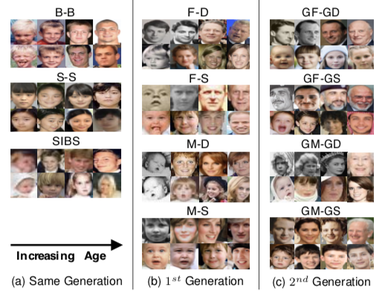
\includegraphics[height=3cm]{facepairs}

There are another smaller family dataset KinFaceW-I and KinFaceW-II, which
includes 533 pairs of parent-child type images.

We divided 95 of the images as training set, 5 percent as test set.

\section{Models and Evaluation}
we use a multi-classifier to indicate what the kinship between two faces is. The
output layer we choose is softmax layer and label could be parent-children,
sibling-sibling or none-kinship.  Triplets training would be used.

FaceNet[2] performs very well in face recognition tasks. We are going to tweak the
model little bits to train our model.

\section*{References}
\medskip
\small
[1] Robinson, Joseph P., et al. Families in the Wild (FIW): Large-Scale Kinship
Image Database and Benchmarks. {\it Proceedings of the 2016 ACM on Multimedia
Conference} - MM '16, 2016, doi:10.1145/2964284.2967219.

[2] Schroff, F., Kalenichenko, D., \& Philbin, J. (2015). FaceNet: A unified
embedding for face recognition and clustering. {\it 2015 IEEE Conference on
Computer Vision and Pattern Recognition (CVPR)}. doi: 10.1109/cvpr.2015.7298682

\end{document}
